%--- MAYO-JUNIO ---
\chapter{Aplicaciones de técnicas avanzadas de Machine Learning y Computación Cuántica en Física de Partículas}

Este capítulo documenta la exploración técnica realizada en el contexto de las 
pruebas de calificación para el programa \textit{Google Summer of Code} (GSoC) 2025. 
El objetivo de estas tareas fue demostrar la competencia en el manejo de circuitos 
cuánticos, el procesamiento de datos físicos mediante grafos y la implementación 
de arquitecturas neuronales de vanguardia.

\section{Introducción a QML-HEP}

La organización \textit{Machine Learning for Science} (ML4SCI) es una iniciativa 
de código abierto que reúne a investigadores de universidades y laboratorios como 
el CERN, con el objetivo de aplicar técnicas modernas de inteligencia artificial a 
problemas complejos en ciencia fundamental \cite{ml4sci}.

Dentro de esta organización, el grupo de trabajo \textit{Quantum Machine Learning 
for High Energy Physics} (QML-HEP) se enfoca específicamente en investigar si la 
computación cuántica puede ofrecer ventajas computacionales —ya sea en velocidad 
o en expresividad— para el análisis de datos provenientes del Gran Colisionador 
de Hadrones (LHC). Las tareas presentadas a continuación fueron diseñadas para 
evaluar la viabilidad técnica de integrar algoritmos cuánticos en flujos de trabajo 
de física de altas energías.

\section{Cumplimiento de la Tarea III: Open Task}

Como parte de los requisitos obligatorios de la evaluación (Task III: Open Task), 
se solicita una discusión original sobre un algoritmo o paradigma de computación 
cuántica que demuestre el entendimiento personal del candidato.

En el contexto de este trabajo, dicho requisito se satisface mediante el análisis 
exhaustivo del \textbf{Algoritmo de Shor} y su implementación práctica, el cual ha 
sido desarrollado en profundidad en el \textbf{Capítulo \ref{cap:shor}} 
(ver página \pageref{cap:shor}). En dicha sección, se discuten no solo los 
fundamentos matemáticos de la transformada cuántica de Fourier y la búsqueda de 
periodo, sino también las implicaciones criptográficas y las limitaciones actuales 
del hardware para su ejecución, cumpliendo así con el objetivo de demostrar 
familiaridad y crítica técnica sobre algoritmos cuánticos fundamentales.

\section{Herramientas de simulación y circuitos cuánticos}

El primer desafío consistió en la implementación de operaciones cuánticas 
fundamentales utilizando dos frameworks prominentes en la industria: 
\textit{Cirq} (desarrollado por Google) y \textit{PennyLane} (desarrollado por 
Xanadu). El dominio de estas herramientas es prerrequisito para diseñar los 
circuitos variacionales que se discutirán más adelante.

\subsection{Fundamentos: Compuertas Hadamard y Controladas}
Los circuitos implementados se basan en un conjunto universal de compuertas que 
manipulan el estado de los qubits en la esfera de Bloch.

\textbf{Compuerta Hadamard ($H$):}
Esta operación es esencial para crear superposición cuántica. Transforma los 
estados de la base computacional $\{|0\rangle, |1\rangle\}$ en estados de 
superposición equiprobable $|+\rangle$ y $|-\rangle$. Matricialmente se define 
como:
\begin{equation}
    H = \frac{1}{\sqrt{2}} \begin{pmatrix} 1 & 1 \\ 1 & -1 \end{pmatrix}
\end{equation}

\textbf{Compuerta CNOT ($CX$):}
La Compuerta Controlada «No» opera sobre dos qubits: un control y un objetivo. 
Invierte el estado del qubit objetivo si y solo si el qubit de control se 
encuentra en el estado $|1\rangle$. Es la operación fundamental para generar 
\textit{entrelazamiento} (entanglement).
\begin{equation}
    CNOT = 
    \begin{pmatrix} 
        1 & 0 & 0 & 0 \\ 
        0 & 1 & 0 & 0 \\ 
        0 & 0 & 0 & 1 \\ 
        0 & 0 & 1 & 0 
    \end{pmatrix}
\end{equation}

\subsection{La operación SWAP y el Test de Intercambio}
La compuerta SWAP intercambia la información cuántica entre dos qubits: 
$|a\rangle|b\rangle \mapsto |b\rangle|a\rangle$. Su representación matricial es:
\begin{equation}
    SWAP = 
    \begin{pmatrix} 
        1 & 0 & 0 & 0 \\ 
        0 & 0 & 1 & 0 \\ 
        0 & 1 & 0 & 0 \\ 
        0 & 0 & 0 & 1 
    \end{pmatrix}
\end{equation}

Más allá de mover información, esta compuerta es la base del \textbf{Swap Test} 
\cite{buhrman2001quantum}, un algoritmo utilizado para medir la fidelidad o 
similitud entre dos estados cuánticos $|\psi\rangle$ y $|\phi\rangle$.

El circuito del Swap Test utiliza un qubit auxiliar (ancilla). Si medimos el 
qubit auxiliar, la probabilidad de encontrarlo en el estado $|0\rangle$ está 
dada por:
\begin{equation}
    P(0) = \frac{1}{2} + \frac{1}{2}|\langle \psi | \phi \rangle|^2
\end{equation}
Donde $|\langle \psi | \phi \rangle|^2$ representa el solapamiento entre los estados. 
Si $P(0)=1$, los estados son idénticos; si $P(0)=0.5$, los estados son ortogonales.

\subsection{Matrices y compuerta de rotación}
Para la codificación de datos clásicos en estados cuánticos y para la construcción 
de circuitos variacionales parametrizados (PQC), se utilizan rotaciones alrededor 
de los ejes de la esfera de Bloch. En la Tarea I, se utilizó específicamente la 
rotación en el eje X, definida por la exponenciación de la matriz de Pauli 
$\sigma_x$:

\begin{equation}
    R_x(\theta) = e^{-i\theta \sigma_x / 2} = 
    \begin{pmatrix} \cos\frac{\theta}{2} & -i\sin\frac{\theta}{2} \\ -i\sin\frac{\theta}{2} & \cos\frac{\theta}{2} \end{pmatrix}
\end{equation}

\subsection{Implementación de circuitos (Tarea 1)}
Para completar esta tarea se desarrollaron dos circuitos distintos 
siguiendo las especificaciones de GSoC.

\subsubsection{Circuito 1: Manipulación de 5 qubits con Cirq}
El primer ejercicio requirió crear un circuito de 5 qubits aplicando superposición 
(Hadamard), entrelazamiento en cadena (CNOTs), intercambio de estados (SWAP) y una 
rotación parametrizada.

\begin{lstlisting}[language=Python, caption=Implementación del primer circuito utilizando Google Cirq.]
import cirq
import numpy as np

# Definicion de 5 qubits
qubits = [cirq.LineQubit(i) for i in range(5)]
circuit = cirq.Circuit()

# 1. Hadamard en todos los qubits
circuit.append(cirq.H(q) for q in qubits)

# 2. CNOT en cadena: (0,1), (1,2), (2,3), (3,4)
circuit.append(cirq.CNOT(qubits[i], qubits[i+1]) for i in range(4))

# 3. SWAP entre el primero (0) y el ultimo (4)
circuit.append(cirq.SWAP(qubits[0], qubits[4]))

# 4. Rotacion Rx(pi/2) en el qubit central (indice 2)
circuit.append(cirq.rx(np.pi / 2)(qubits[2]))

print(circuit)
\end{lstlisting}

La ejecución de este código genera un diagrama del circuito donde se verifica la 
estructura lineal de las compuertas CNOT y la rotación final. podemos visualizar el
circuito resultante en la Figura \ref{fig:cirq_circuit_1}.

\begin{figure}[H]
        \centering
        \includegraphics[width=0.75\linewidth]{imagenes/Cirq_1_circuit.png}
        \caption{circuito resultante del código con cirq para aplicar el primer 
        conjunto de compuertas.}
        \label{fig:cirq_circuit_1}
\end{figure}

\subsubsection{Circuito 2: Swap Test con PennyLane}
El segundo ejercicio consistió en implementar un \textit{Swap Test} entre dos 
pares de qubits. Se prepararon los estados aplicando Hadamards y una rotación 
$R_x(\pi/3)$ para diferenciar los subsistemas, y luego se midió su similitud.

\begin{lstlisting}[language=Python, caption=Implementación del Swap Test 
    utilizando PennyLane]
import pennylane as qml
import numpy as np

# 5 qubits: 1 ancilla + 4 para el sistema
dev = qml.device("default.qubit", wires=5)

@qml.qnode(dev, interface="autograd")
def swap_test_circuit():
    ancilla = 0
    q1, q2 = 1, 2
    q3, q4 = 3, 4

    # --- Preparacion de Estados ---
    qml.Hadamard(wires=q1)       # Estado A parte 1
    qml.RX(np.pi/3, wires=q2)    # Estado A parte 2
    qml.Hadamard(wires=q3)       # Estado B parte 1
    qml.Hadamard(wires=q4)       # Estado B parte 2

    # --- Rutina de Swap Test ---
    qml.Hadamard(wires=ancilla)
    
    # SWAP Controlado entre los pares (q1,q3) y (q2,q4)
    qml.CSWAP(wires=[ancilla, q1, q3])
    qml.CSWAP(wires=[ancilla, q2, q4])

    qml.Hadamard(wires=ancilla)

    return qml.probs(wires=ancilla)

probs = swap_test_circuit()
print(f"Probabilidad P(0): {probs[0]:.4f}")
\end{lstlisting}

\subsection{Comparación de paradigmas: PennyLane vs Cirq}
Tras la implementación de ambos ejercicios, se identificaron diferencias clave 
en la filosofía de diseño de ambos frameworks:

\begin{itemize}
    \item \textbf{Cirq (Enfoque de Hardware):} Cirq opera a un nivel de abstracción 
    más bajo\cite{cirq}. Su estructura permite definir qubits específicos (como GridQubit 
    para chips Sycamore) y momentos temporales precisos. Es ideal para algoritmos 
    canónicos como Shor (visto en capítulos anteriores) donde la secuencia exacta 
    de compuertas es crítica.
    
    \item \textbf{PennyLane (Enfoque de Software/ML):} Como se observa en el 
    decorador @qml.qnode(..., interface='autograd'), PennyLane está diseñado 
    para la \textbf{Programación Diferenciable} \cite{bergholm2018pennylane}. 
    Trata a los circuitos cuánticos 
    como nodos en un grafo computacional que pueden ser derivados automáticamente. 
    Esto lo hace superior para tareas de Aprendizaje Automático Cuántico (QML), 
    donde es necesario calcular gradientes de los parámetros de rotación (como el 
    ángulo $\pi/3$ en el ejemplo) para optimizar funciones de costo mediante 
    descenso de gradiente.
\end{itemize}

\section{Aprendizaje profundo geométrico: GNN en física}

La física de altas energías, y otras ramas como la química cuántica, comparten un 
desafío fundamental en el análisis de datos: la naturaleza no estructurada y 
relacional de sus sistemas.
A diferencia de las imágenes, que poseen una estructura de cuadrícula euclidiana 
fija, o del texto, que es secuencial, los sistemas físicos —como moléculas o 
chorros de partículas (jets)— se representan mejor como entidades discretas 
interactuantes distribuidas en un espacio métrico. El Aprendizaje Profundo 
Geométrico (\textit{Geometric Deep Learning}) proporciona el marco teórico 
para abordar estos dominios irregulares, siendo las Redes Neuronales de Grafos 
(GNN) su exponente más exitoso.

\subsection{Fundamentos de grafos}

Un grafo es una estructura matemática que modela un conjunto de objetos y las 
relaciones entre ellos. Formalmente, definimos un grafo $G$ como una tupla 
$G = (V, E)$, donde $V$ es el conjunto de vértices o nodos y $E$ representa el 
conjunto de aristas que conectan pares de nodos.

En el contexto del aprendizaje automático aplicado a la física, extendemos esta 
definición para incluir atributos, \textit{features}, asociados a cada componente
del grafo:

\begin{itemize}
    \item \textbf{Atributos de Nodo ($\mathbf{h}_v$):} Cada nodo $v \in V$ tiene 
    asociado un vector de características $\mathbf{h}_v \in \mathbb{R}^{d_v}$, 
    que describe el estado local de la entidad, por ejemplo el tipo de átomo, 
    momento de una partícula.
    \item \textbf{Atributos de Arista ($\mathbf{e}_{vw}$):} Cada arista $(v, w) 
    \in E$ puede tener un vector de características $\mathbf{e}_{vw} \in 
    \mathbb{R}^{d_e}$, que codifica la relación entre los nodos, por ejemplo 
    la distancia espacial o el tipo de enlace químico.
    \item \textbf{Atributos Globales ($\mathbf{u}$):} Opcionalmente, el grafo 
    puede tener un vector global $\mathbf{u}$ que representa propiedades del 
    sistema completo.
\end{itemize}

La estructura conectiva del grafo se puede representar mediante la matriz de 
adyacencia $\mathbf{A} \in \{0, 1\}^{|V| \times |V|}$, donde $a_{ij} = 1$ si 
existe una arista entre el nodo $i$ y el nodo $j$, y $0$ en caso contrario.

Las GNNs operan sobre esta estructura aprovechando una propiedad clave para la 
física: la \textbf{invariancia a las permutaciones}. Dado que no existe un orden 
canónico para enumerar las partículas en una colisión o los átomos en una 
molécula, cualquier función de aprendizaje $f(G)$ debe cumplir que 
$f(\mathbf{P}\mathbf{A}\mathbf{P}^T, \mathbf{P}\mathbf{H}) = f(\mathbf{A}, 
\mathbf{H})$ para cualquier matriz de permutación $\mathbf{P}$. Esto asegura 
que las predicciones físicas no dependan del orden arbitrario de entrada de 
los datos.

\subsection{Representación de jets como grafos}

En física de altas energía, particularmente cuando se trabaja con colisionadores, 
un \textit{jet} es un chorro colimado de hadrones 
producido por la hadronización de un quark o gluón de alta energía. 
Tradicionalmente, los jets se han analizado proyectando su energía en una 
cuadrícula (imágenes calorimétricas) o tratándolos como secuencias. Sin embargo, 
estas representaciones imponen una estructura artificial o pierden información 
sobre la dispersión natural de las partículas.

Una representación más natural a la física del proceso es considerar el jet como una 
«nube de puntos» o un grafo. Definimos formalmente un jet como un grafo 
dirigido $G_{jet} = (V, E)$ de la siguiente manera:

\begin{itemize}
    \item \textbf{Nodos ($V$):} Cada nodo representa una partícula constituyente 
    del jet. El vector de características inicial del nodo $i$, denotado 
    como $\mathbf{h}_i^{(0)}$, incluye variables cinemáticas fundamentales:
    \begin{equation}
        \mathbf{h}_i^{(0)} = (\Delta\eta_i, \Delta\phi_i, \log p_{T,i}, 
        \dots)
    \end{equation}
    Donde $\Delta\eta_i$ y $\Delta\phi_i$ son las coordenadas de 
    pseudorapidez y ángulo azimutal relativas al eje del jet, y $p_{T,i}$ 
    es el momento transversal.

    \item \textbf{Aristas ($E$):} La topología del grafo se construye 
    dinámicamente para capturar correlaciones locales. Comúnmente se 
    utiliza el algoritmo de $k$-vecinos más cercanos ($k$-NN). Para cada 
    partícula $i$, se establecen aristas dirigidas $e_{ij} \in E$ hacia sus $k$ 
    vecinos más cercanos en el espacio $(\Delta\eta, \Delta\phi)$. El peso o 
    característica de la arista $\mathbf{e}_{ij}$ se define mediante la métrica 
    euclidiana en este espacio:
    \begin{equation}
        \mathbf{e}_{ij} = \sqrt{(\Delta\eta_i - \Delta\eta_j)^2 + 
        (\Delta\phi_i - \Delta\phi_j)^2}
    \end{equation}
\end{itemize}

Esta representación permite que la red neuronal aprenda directamente de la 
estructura de la lluvia de partículas (\textit{parton shower}), donde las 
partículas cercanas en el espacio angular están probablemente relacionadas 
por el mismo proceso de desintegración.

\begin{figure}[H]
    \centering
    \includegraphics[width=0.8\linewidth]{imagenes/jet_graph_representation.png}
    \caption{Ilustración de la transformación de un evento de colisión a una 
    representación de grafo. Las partículas (nodos) se conectan con sus vecinos 
    espaciales más cercanos (aristas), formando una estructura irregular que 
    preserva la geometría del evento.}
    \label{fig:jet_graph}
\end{figure}

\subsection{Formalismo del Paso de Mensajes (Message Passing)}

El marco teórico que unifica la mayoría de las arquitecturas de GNN modernas es 
el de las \textit{Message Passing Neural Networks} (MPNN), formalizado por 
Gilmer et al. (2017) en el contexto de la química cuántica. Este formalismo 
describe el proceso de aprendizaje como un intercambio iterativo de información 
entre nodos a través de las aristas.

El algoritmo de paso de mensajes se ejecuta durante $T$ pasos temporales. 
En cada paso $t$, el estado oculto de cada nodo $\mathbf{h}_v^t$ se actualiza 
basándose en su estado anterior y en la agregación de los mensajes recibidos 
de su vecindario $\mathcal{N}(v)$. El proceso se define mediante dos funciones 
diferenciables principales: la función de mensaje $M_t$ y la función de 
actualización $U_t$.

\textbf{1. Fase de Mensaje y Agregación:}
Para cada nodo $v$, se calcula un mensaje agregado $\mathbf{m}_v^{t+1}$ sumando 
la información proveniente de sus vecinos:
\begin{equation}
    \mathbf{m}_v^{t+1} = \sum_{w \in \mathcal{N}(v)} M_t(\mathbf{h}_v^t, 
    \mathbf{h}_w^t, \mathbf{e}_{vw})
    \label{eq:message_passing}
\end{equation}
Donde:
\begin{itemize}
    \item $M_t$ es una red neuronal (típicamente un perceptrón multicapa o MLP) 
    que computa la interacción entre el nodo $v$, su vecino $w$ y la arista que 
    los une.
    \item La sumatoria $\sum$ actúa como un operador de agregación invariante a 
    permutaciones, asegurando que el resultado no dependa del orden en que se 
    procesan los vecinos.
\end{itemize}

\textbf{2. Fase de Actualización:}
El estado del nodo se actualiza combinando su estado actual con el mensaje agregado:
\begin{equation}
    \mathbf{h}_v^{t+1} = U_t(\mathbf{h}_v^t, \mathbf{m}_v^{t+1})
    \label{eq:update_function}
\end{equation}
Donde $U_t$ suele ser una red neuronal recurrente (como una GRU o LSTM) o 
simplemente otra capa densa.

\textbf{3. Fase de Lectura (Readout):}
Después de $K$ iteraciones de paso de mensajes, la información local se ha 
propagado por el grafo. Para tareas de clasificación a nivel de grafo (como 
distinguir si un jet es quark o gluón), se utiliza una función de lectura $R$ 
para generar una predicción global $\hat{y}$:
\begin{equation}
    \hat{y} = R(\{\mathbf{h}_v^K | v \in G\})
\end{equation}

La función $R$ debe ser también invariante al orden de los nodos, por ejemplo la
suma global o promedio global. Este formalismo permite modelar interacciones 
complejas de muchos cuerpos mediante la composición 
de interacciones locales simples.

\begin{figure}[H]
    \centering
    \includegraphics[width=0.9\linewidth]{imagenes/mpnn_diagram.png}
    \caption{Diagrama esquemático de una capa de Message Passing. (A) Los nodos 
    vecinos envían mensajes a través de las aristas. (B) Los mensajes se agregan 
    (suma). (C) El estado del nodo central se actualiza con la información agregada.}
    \label{fig:mpnn_scheme}
\end{figure}

\subsection{Mecanismo de atención (GAT)}

Una limitación de las MPNN básicas es que el operador de agregación (Ec. 
\ref{eq:message_passing}) suele tratar a todos los vecinos por igual o basarse 
únicamente en características estáticas de la arista. En física de partículas, 
sin embargo, no todas las interacciones son igual de relevantes; una partícula 
con alto momento transversal ($p_T$) cercana al eje del jet puede contener mucha 
más información sobre el proceso original que una partícula de baja energía en la 
periferia.

Para incorporar esta intuición física, empleamos las Redes de Atención de Grafos 
(Graph Attention Networks, GAT). Las GAT introducen un mecanismo de atención que 
permite a la red aprender \textit{qué} vecinos son más importantes para la 
actualización de un nodo específico.

El núcleo de la GAT es el cálculo de los coeficientes de atención $\alpha_{ij}$. 
Primero, se calcula un puntaje de importancia no normalizado $e_{ij}$ entre el 
nodo $i$ y su vecino $j$:
\begin{equation}
    e_{ij} = \text{LeakyReLU}\left( \mathbf{a}^T [\mathbf{W}\mathbf{h}_i \| 
    \mathbf{W}\mathbf{h}_j] \right)
\end{equation}
Donde:
\begin{itemize}
    \item $\mathbf{W}$ es una matriz de transformación lineal aprendible 
    aplicada a cada nodo.
    \item $\mathbf{a}$ es el vector de parámetros del mecanismo de atención.
    \item $\|$ denota la concatenación de vectores.
    \item LeakyReLU es la función de activación que permite gradientes para 
    valores negativos.
\end{itemize}

Para hacer los coeficientes comparables entre diferentes nodos, se normalizan 
utilizando la función softmax sobre todos los vecinos $k \in \mathcal{N}(i)$:
\begin{equation}
    \alpha_{ij} = \frac{\exp(e_{ij})}{\sum_{k \in \mathcal{N}(i)} \exp(e_{ik})}
    \label{eq:attention_coeff}
\end{equation}

Finalmente, la agregación de mensajes se convierte en una suma ponderada por 
estos coeficientes:
\begin{equation}
    \mathbf{h}_i' = \sigma \left( \sum_{j \in \mathcal{N}(i)} \alpha_{ij} 
    \mathbf{W}\mathbf{h}_j \right)
\end{equation}

En el contexto de la física de jets, el coeficiente $\alpha_{ij}$ puede 
interpretarse como la importancia relativa de la partícula $j$ para determinar 
la naturaleza de la partícula $i$. Esto permite que el modelo filtre el ruido de 
fondo y se enfoque en las partículas energéticas que definen la 
subestructura del jet, mejorando significativamente la capacidad de clasificación 
y proporcionando interpretabilidad al modelo.

\subsection{Implementación y resultados}

Para evaluar la eficacia de las arquitecturas geométricas propuestas, se implementó 
un flujo de trabajo completo en \textit{PyTorch Geometric}, abarcando desde la 
ingestión de datos crudos hasta la validación de los modelos MPNN y GAT.

\subsubsection{Base de datos usada: ParticleNet}

El estudio utilizó el conjunto de datos estándar de \textbf{ParticleNet} para la 
clasificación de jets de quarks y gluones. Este dataset consta de eventos simulados 
con el generador Pythia, proporcionando una representación de «nube de puntos» 
ideal para el aprendizaje basado en grafos.

\textbf{Características del Dataset:}
\begin{itemize}
    \item \textbf{Volumen:} El conjunto total consta de 100,000 eventos, 
    balanceados equitativamente entre jets de quarks (señal) y jets de gluones 
    (fondo).
    \item \textbf{Atributos de Entrada:} Cada jet está compuesto por una lista de 
    partículas, donde cada partícula posee cuatro características fundamentales:
    \begin{itemize}
        \item Momento transversal ($p_T$).
        \item Rapidez ($y$).
        \item Ángulo azimutal ($\phi$).
        \item Identificador de partícula (pdgid).
    \end{itemize}
    \item \textbf{Preprocesamiento y Construcción del Grafo:}
    Dado que los jets tienen una multiplicidad variable, los datos originales 
    incluyen padding (relleno con ceros). Para la construcción del grafo, se 
    implementó un filtro, threshold=1e-6, para descartar estas partículas 
    ficticias.
    
    A diferencia de los enfoques estáticos, se optó por una topología de 
    \textbf{Grafo Totalmente Conectado} para cada jet. Esto significa que cada 
    partícula (nodo) tiene una arista dirigida hacia todas las demás partículas 
    del jet. Si bien esto incrementa el costo computacional respecto a un enfoque 
    de $k$-vecinos más cercanos ($k$-NN), permite que el mecanismo de paso de 
    mensajes capture interacciones globales de largo alcance dentro del cono del 
    jet, delegando a la red neuronal la tarea de aprender qué conexiones son 
    relevantes.
\end{itemize}

\textbf{División de Datos:}
Se utilizaron dos archivos \textit{.npz} para el entrenamiento y validación 
(\textit{QG\_jets.npz}, \textit{QG\_jets\_11.npz}), 
reservando un tercer archivo independiente (\textit{QG\_jets\_12.npz}) 
exclusivamente para la evaluación final (Test Set).

\subsubsection{Resultados}

El entrenamiento se realizó utilizando el optimizador \textbf{Adam} con una 
tasa de aprendizaje inicial de $10^{-3}$ y un decaimiento de pesos 
(\textit{weight decay}) de $5 \times 10^{-4}$ para regularización L2. 
Se implementó una estrategia de \textit{Early Stopping} monitoreando la 
pérdida de validación, con una paciencia de 4 épocas para prevenir el 
sobreajuste y optimizar el uso de recursos.

Ambos modelos lograron converger, aunque exhibieron dinámicas de aprendizaje 
marcadamente distintas:
\begin{itemize}
    \item \textbf{Eficiencia Computacional:} La arquitectura MPNN fue 
    notablemente más rápida en completar su entrenamiento. Debido a su 
    simplicidad operativa, agregación por suma; cada época requirió menos 
    tiempo de cómputo en comparación con la GAT, cuyo mecanismo de atención 
    tiene una complejidad cuadrática $O(N^2)$ respecto al número de nodos en 
    el grafo totalmente conectado.
    \item \textbf{Dinámica de Aprendizaje:} La MPNN mostró una convergencia 
    rápida y estable, activando el criterio de parada temprana en la época 7, 
    tras dejar de mejorar en la época 3. Por el contrario, la GAT continuó 
    ajustando sus pesos más lentamente, alcanzando su mejor rendimiento hacia 
    la época 6, lo que evidencia una superficie de optimización más compleja 
    debido a los coeficientes de atención.
\end{itemize}

Para visualizar el desempeño detallado de cada clasificador, presentamos 
las matrices de confusión normalizadas calculadas sobre el conjunto de prueba.

\begin{figure}[H]
    \centering
    \begin{minipage}{0.48\textwidth}
        \centering
        \includegraphics[width=0.9\linewidth]{imagenes/matriz_confusion_MPNN.png}
        \caption{Matriz de confusión MPNN.}
        \label{fig:mpnn_matriz_confusion}
    \end{minipage}\hfill
    \begin{minipage}{0.48\textwidth}
        \centering
        \includegraphics[width=0.9\linewidth]{imagenes/matriz_confusion_GAT.png}
        \caption{Matriz de confusión GAT.}
        \label{fig:conf_matrix_gat}
    \end{minipage}
\end{figure}

\begin{figure}[H]
    \centering
    \begin{minipage}{0.48\textwidth}
        \centering
        % Representación tabular de la matriz de confusión para MPNN
        % Datos crudos: TP_g=37776, FP_q=12224, FN_q=10717, TP_q=39283
        \begin{tabular}{|c|c|c|}
            \hline
            \textbf{MPNN} & Pred: Gluón & Pred: Quark \\
            \hline
            Real: Gluón & \textbf{TP$_{g}$: 75.6\%} & FP$_{q}$: 24.4\% \\
            \hline
            Real: Quark & FN$_{q}$: 21.4\% & \textbf{TP$_{q}$: 78.6\%} \\
            \hline
        \end{tabular}
        \caption{Matriz de confusión MPNN normalizada.}
        \label{fig:conf_matrix_mpnn_normalizada}
    \end{minipage}\hfill
    \begin{minipage}{0.48\textwidth}
        \centering
        % Representación tabular de la matriz de confusión para GAT
        % Datos crudos: TP_g=43707, FP_q=6293, FN_q=17056, TP_q=32944
        \begin{tabular}{|c|c|c|}
            \hline
            \textbf{GAT} & Pred: Gluón & Pred: Quark \\
            \hline
            Real: Gluón & \textbf{TP$_{g}$: 87.4\%} & FP$_{q}$: 12.6\% \\
            \hline
            Real: Quark & FN$_{q}$: 34.1\% & \textbf{TP$_{q}$: 65.9\%} \\
            \hline
        \end{tabular}
        \caption{Matriz de confusión GAT normalizada.}
        \label{fig:conf_matrix_gat_normalizada}
    \end{minipage}
\end{figure}

\textbf{Análisis de Métricas:}
La Tabla \ref{tab:gnn_comparison} resume las métricas finales en el conjunto de 
prueba. Si bien la exactitud global (\textit{Accuracy}) es comparable entre ambos 
modelos ($\approx 77\%$), la distribución de los errores revela especializaciones 
opuestas:

\begin{itemize}
    \item La \textbf{GAT} prioriza la \textbf{Precisión} (83.96\%), minimizando 
    drásticamente los Falsos Positivos de quarks, solo 12.6\% de gluones mal clasificados. 
    Esto indica que el mecanismo de atención aprende a filtrar el ruido de fondo 
    eficazmente.
    \item La \textbf{MPNN} prioriza el \textbf{Recall} (78.57\%), maximizando la 
    detección de quarks reales, aunque a costa de una menor pureza, mayor 
    contaminación por gluones.
\end{itemize}

\begin{table}[H]
    \centering
    \begin{tabular}{|l| c c c c|}
        \toprule
        \textbf{Modelo} & \textbf{Accuracy} & \textbf{Precision} & \textbf{Recall} & \textbf{Training Time} \\
        \midrule
        MPNN (Message Passing) & 0.7706 & 0.7627 & \textbf{0.7857} & $\approx$ 2h 11m \\
        GAT (Graph Attention) & 0.7665 & \textbf{0.8396} & 0.6589 & $>$ 4h \\
        \bottomrule
    \end{tabular}
    \caption{Comparación de rendimiento entre arquitecturas GNN en el dataset 
    de prueba ParticleNet.}
    \label{tab:gnn_comparison}
\end{table}

Estos resultados confirman que la topología del grafo contiene bien la información 
física: la GAT explota las correlaciones fuertes para asegurar predicciones 
de alta confianza, mientras que la MPNN utiliza la información global agregada 
para no perder señales potenciales.

\subsubsection{Discusión}

El análisis comparativo permite establecer criterios claros para la selección del 
modelo según el objetivo físico del análisis:

\textbf{1. Compromiso Precisión-Recall (Pureza vs. Eficiencia)}
\begin{itemize}
    \item \textbf{GAT para Alta Pureza:} Con una precisión cercana al 84\%, la 
    GAT es la arquitectura ideal para mediciones de precisión donde es crítico 
    que la muestra de quarks esté libre de contaminación por gluones, aun si 
    eso implica descartar algunos eventos válidos.
    \item \textbf{MPNN para Máxima Eficiencia:} Con un recall del 78.6\%, la 
    MPNN es superior para búsquedas de señales exóticas o raras, búsqueda de 
    nueva física; donde el costo de perder un evento de señal 
    es inaceptable y se tolera un mayor ruido de fondo.
\end{itemize}

\textbf{2. Costo computacional y escalabilidad}
\begin{itemize}
    \item \textbf{Escalabilidad de GAT:} El costo cuadrático de la atención limita 
    su uso en grafos muy densos o en entornos con recursos limitados.
    \item \textbf{Viabilidad de MPNN:} Su convergencia rápida y menor huella 
    computacional la hacen candidata para despliegues en tiempo real, como en los 
    sistemas de selección de eventos del LHC, donde la latencia 
    es un factor crítico.
\end{itemize}

\subsubsection{Conclusiones y trabajo futuro}

El estudio realizado demuestra que las arquitecturas basadas en grafos, tanto 
MPNN como GAT, logran explotar exitosamente la estructura geométrica intrínseca 
de los datos de jets en \textit{ParticleNet}, superando las limitaciones de los 
enfoques tradicionales que dependen de variables de alto nivel pre-calculadas.

La comparación directa revela una dicotomía clara en la aplicación de estos modelos:
\begin{itemize}
    \item La \textbf{GAT (Graph Attention Network)} se establece como la 
    herramienta superior para tareas de \textbf{alta pureza}. Su capacidad para 
    asignar pesos de importancia a las partículas más relevantes le permite filtrar 
    el ruido de fondo con gran eficacia, logrando una precisión del 83.96\% en la 
    identificación de quarks.
    \item La \textbf{MPNN (Message Passing Neural Network)} destaca por su 
    \textbf{eficiencia de señal} y velocidad. Al capturar una mayor cantidad de 
    quarks reales (Recall del 78.57\%) con un costo computacional significativamente 
    menor, se presenta como la opción viable para análisis donde la estadística 
    es prioritaria sobre la pureza.
\end{itemize}

La elección entre una y otra no es absoluta, sino que debe guiarse por los 
requisitos específicos del análisis físico: minimizar falsos positivos (GAT) o 
maximizar la eficiencia de detección (MPNN).

A partir de los hallazgos de esta investigación, se identifican tres líneas 
principales para extender y mejorar el uso de GNNs en física de altas energías:

\begin{enumerate}
    \item \textbf{Exploración de representaciones de grafo alternativas:}
    Actualmente, la topología totalmente conectada asegura que no se pierda 
    información, pero a un alto costo. Futuros trabajos podrían investigar 
    métodos de construcción de grafos más sofisticados, como el uso de 
    umbrales de distancia dinámica ($\Delta R < R_{cut}$) o métricas de similitud 
    inspiradas en la física, por ejemplo la invariancia de Lorentz; para definir 
    las aristas, reduciendo la complejidad computacional sin sacrificar la física.

    \item \textbf{Mejoras en la arquitectura del modelo:}
    Se propone investigar arquitecturas con mayor poder expresivo teórico, como 
    las \textit{Graph Isomorphism Networks} (GIN), o desarrollar modelos híbridos 
    que combinen la eficiencia del paso de mensajes en las primeras capas 
    (para agregación local) con la selectividad de la atención en las capas 
    profundas (para razonamiento global).

    \item \textbf{Optimización de hiperparámetros:}
    Debido a las restricciones de tiempo del ejercicio, la exploración del 
    espacio de hiperparámetros fue limitada. Un estudio de ablación exhaustivo y
    una sintonización fina (\textit{fine-tuning}) de parámetros como la dimensión 
    del espacio latente, el número de cabezas de atención y las tasas de 
    \textit{dropout} podrían desbloquear un rendimiento superior en la clasificación.
\end{enumerate}

\section{Redes neuronales Kolmogorov-Arnold (KAN)}

Durante la última década, el Perceptrón Multicapa (MLP) ha permanecido como la 
unidad fundamental del aprendizaje profundo. Basado en el \textit{Teorema de Aproximación 
Universal}, los MLPs han demostrado ser increíblemente buenos en aproximar 
funciones no lineales en espacios de varias dimensiones. Sin embargo, recientemente 
se ha propuesto un cambio de paradigma inspirado en un resultado fundamental de 
la teoría de funciones de los años 50: las Redes de Kolmogorov-Arnold, KAN.

A diferencia de las redes tradicionales que fijan las funciones de activación en 
los nodos (neuronas) y aprenden pesos lineales en las aristas, las KANs invierten 
esta lógica, colocando funciones de activación aprendibles en las aristas y 
utilizando nodos como sumatorios simples. Este enfoque, propuesto formalmente 
para el aprendizaje automático por Liu et al. (2025) \cite{liu2025kan}, 
promete ventajas significativas en términos de interpretabilidad y eficiencia 
de parámetros para tareas científicas.

\subsection{El teorema de Kolmogorov-Arnold}

\subsubsection{Teorema y explicación}
El fundamento matemático de esta arquitectura reside en el \textbf{Teorema de 
Representación de Kolmogorov-Arnold}. Originalmente formulado por Andrey 
Kolmogorov (1957) \cite{kolmogorov1957representation} y refinado por Vladimir 
Arnold, este teorema resolvió el decimotercer problema de Hilbert, demostrando 
que cualquier función continua multivariada puede reducirse a una composición 
finita de funciones continuas de una sola variable y la operación de suma.

\textbf{Teorema} 

Para cualquier función continua multivariada $f: [0,1]^n \to \mathbb{R}$, 
existen funciones continuas univariadas $\Phi_q: \mathbb{R} \to \mathbb{R}$ y 
$\phi_{q,p}: [0,1] \to \mathbb{R}$ tales que:

\begin{equation}
    f(x_1, \dots, x_n) = \sum_{q=0}^{2n} \Phi_q \left( \sum_{p=1}^n 
    \phi_{q,p}(x_p) \right)
    \label{eq:kolmogorov_theorem}
\end{equation}

Donde:
\begin{itemize}
    \item $n$ es la dimensión de la entrada.
    \item $x_p$ es la $p$-ésima componente del vector de entrada $\mathbf{x}$.
    \item $\phi_{q,p}$ son las funciones internas que 
    transforman cada coordenada individualmente.
    \item $\Phi_q$ son las funciones externas que 
    procesan la suma de las transformaciones internas.
    \item La sumatoria externa se realiza sobre $2n+1$ términos.
\end{itemize}

Históricamente, este teorema fue considerado una curiosidad teórica en el 
contexto de la aproximación numérica \cite{schmidt2021kolmogorov}. 
La razón es que las funciones internas $\phi_{q,p}$ garantizadas por el teorema 
suelen ser no suaves, como los fractales, y altamente dependientes de la función 
objetivo $f$ específica, lo que las hacía inútiles para el aprendizaje constructivo. 
Sin embargo, la innovación de las KANs modernas radica en relajar la restricción 
de usar exactamente $2n+1$ términos y, en su lugar, parametrizar estas funciones 
univariadas como curvas suaves, \textit{splines}, que pueden aprenderse mediante 
descenso de gradiente.

\begin{figure}[H]
    \centering
    \includegraphics[width=0.9\linewidth]{imagenes/Flujo_KAN.png}
    \caption{Representación esquemática del Teorema de Kolmogorov-Arnold. 
    Cada entrada $x_p$ pasa por funciones univariadas no lineales $\phi$ antes 
    de ser sumada.
    Izquierda: Notaciones de las activaciones que fluyen a través de la red. 
    Derecha: Una función de activación está parametrizada como B-spline, lo que 
    permite alternar entre cuadrículas gruesas y finas. Imagen 
    extraída de liu et al. (2025) \cite{liu2025kan}.}
    \label{fig:ka_theorem}
\end{figure}

\subsubsection{Comparación con MLP y el teorema de aproximación universal}

La diferencia estructural entre un perceptrón multicapa, MLP, y una KAN es 
profunda y radica en dónde reside la no-linealidad aprendible.

\textbf{1. El enfoque MLP (activación en nodos):}

Un MLP se basa en el Teorema de Aproximación Universal de Cybenko 
\cite{cybenko1989approximation}, el cual establece que una red con suficiente 
profundidad puede aproximar cualquier función. Estructuralmente, el procesamiento 
en un MLP ocurre en dos etapas: primero se realiza una \textbf{combinación lineal} 
de las entradas (mediante una matriz de pesos $W$) y posteriormente se aplica una 
función de activación no lineal fija $\sigma$ (como ReLU o Sigmoide):

\begin{equation}
    f_{MLP}(\mathbf{x}) = \sigma \left( \sum_{j=1}^{d_{in}} w_{ij} x_j + b_i \right)
\end{equation}

Aquí, los parámetros aprendibles son los pesos lineales $w_{ij}$ y los sesgos $b_i$. 
La función $\sigma$ es estática y no evoluciona durante el entrenamiento. 
Esto limita la expresividad de cada neurona individual, obligando a la red a 
incrementar su número de neuronas para modelar comportamientos complejos.

\textbf{2. El enfoque KAN (activación en aristas):}

Una KAN generaliza la Ec. \ref{eq:kolmogorov_theorem} a capas arbitrarias de 
profundidad. En una capa KAN, la transformación entre la capa $l$ y $l+1$ se 
define como:
\begin{equation}
    x_i^{(l+1)} = \sum_{j=1}^{n_l} \phi_{l,j,i} (x_j^{(l)})
\end{equation}
Aquí, $\phi_{l,j,i}$ no es un peso escalar, sino una \textbf{función univariada 
aprendible} que conecta el nodo $j$ de la capa anterior con el nodo $i$ de la 
capa actual.

Esta distinción tiene consecuencias críticas:
\begin{itemize}
    \item \textbf{Eficiencia de Parámetros:} Mientras que un MLP necesita apilar 
    muchas capas y neuronas para aproximar una función compleja, como una 
    multiplicación o una función oscilatoria; una KAN puede aprender la función 
    exacta en las aristas. Por ejemplo, una KAN puede aprender $f(x,y) = xy$ 
    usando la identidad logarítmica $\log(xy) = \log x + \log y$, reduciendo la 
    red a sumas y funciones $\phi(x)=\log(x)$ y $\Phi(x)=\exp(x)$, algo 
    extremadamente difícil para un MLP estándar \cite{liu2025kan}.
    \item \textbf{Interpretabilidad:} En un MLP, los pesos $W$ son matrices 
    densas difíciles de interpretar. En una KAN, cada conexión es una función 
    $y = \phi(x)$ que puede visualizarse gráficamente. Si una conexión aprende 
    una función cercana a cero, puede podarse; si aprende una curva cuadrática, 
    puede sustituirse simbólicamente por $x^2$.
\end{itemize}

\begin{figure}[H]
    \centering
    \begin{tabular}{|c|c|c|}
            \hline
            modelo 
            & \textbf{Perceptrón multicapa (MLP)} 
            & \textbf{Red Kolmogorov-Arnold (KAN)} \\
            \hline
            Teorema & Teorema de aproximación universal & Teorema de representación Kolmogorov Arnold \\
            \hline
            Fórmula 
            & $f(\mathbf{x}) \approx \sum^{N(\epsilon)}_{i=1} a_i \sigma(\mathbf{w}_i \cdot \mathbf{x} + b_i)$ 
            & $f(x) = \sum^{2n+1}_{q=1} \Phi_q \left( \sum^{n}_{p=1} \phi_{q,p}(x_p) \right)$ \\
            \hline
            Modelo 
            & \includegraphics[width=0.35\linewidth]{imagenes/MLP_esquema.png} 
            & \includegraphics[width=0.35\linewidth]{imagenes/KAN_esquema.png} \\
            \hline
        \end{tabular}
    \caption{Comparación arquitectónica. (Izquierda) MLP: Las aristas son pesos 
    lineales $w$ y los nodos aplican la no-linealidad $\sigma$. (Derecha) KAN: 
    Las aristas contienen funciones aprendibles $\phi$ y los nodos simplemente 
    suman las señales entrantes. Imagen extraída de liu et al. (2025) 
    \cite{liu2025kan}.}
    \label{fig:mlp_vs_kan}
\end{figure}


\subsection{B-splines y capas densas}

Para implementar computacionalmente las funciones $\phi(x)$ descritas en el 
teorema, no podemos optimizar en el espacio de todas las funciones continuas. 
Debemos restringirnos a un espacio paramétrico flexible. Liu et al. proponen el 
uso de \textbf{B-splines} (Basis Splines).

Una función de activación en una KAN se parametriza como la suma de una función 
base, para regularización y estabilidad, y una combinación lineal de funciones 
B-spline:

\begin{equation}
    \phi(x) = w_b b(x) + w_s \text{spline}(x)
\end{equation}

Donde:
\begin{itemize}
    \item $b(x)$ es una función de activación base, típicamente la función 
    SiLU ($x / (1 + e^{-x})$).
    \item $w_b, w_s$ son factores de escala aprendibles.
    \item $\text{spline}(x)$ se expresa como una combinación lineal de $k$ 
    funciones base B-spline $B_i(x)$ definidas en una retícula (\textit{grid}) de 
    puntos de control $c_i$:
    \begin{equation}
        \text{spline}(x) = \sum_{i} c_i B_i(x)
    \end{equation}
\end{itemize}

\textbf{Optimización y extensión de la cuadrícula (Grid Extension)}

Los coeficientes $c_i$ son los parámetros que se actualizan mediante descenso de 
gradiente. Una ventaja clave de los B-splines es su localidad: modificar un 
coeficiente $c_i$ solo afecta la forma de la función en un intervalo local, 
evitando el «olvido» global que sufren los MLPs.

Además, esta parametrización permite una propiedad única llamada \textit{Grid 
Extension}. Se puede comenzar entrenando una KAN con una retícula gruesa, 
pocos puntos de control, pocos parámetros; para aprender la estructura global 
de la función, y luego refinar la retícula añadiendo más puntos de control, 
inicializando sus valores para preservar la forma de la función aprendida. 
Esto permite escalar la precisión del modelo sin reentrenar desde cero, algo 
imposible en arquitecturas densas tradicionales.

\textbf{Capas KAN (KANLinear):}
En la implementación práctica (usando PyTorch), una Capa KAN sustituye a la capa 
lineal convencional (\textit{nn.Linear}). Dado un batch de entrada $\mathbf{X}$ de 
dimensión $(Batch, N_{in})$, la capa calcula la salida $(Batch, N_{out})$ 
evaluando todos los B-splines correspondientes a las $N_{in} \times N_{out}$ 
aristas y sumando los resultados. Aunque computacionalmente más costoso que una 
simple multiplicación matricial debido a la evaluación de los polinomios spline, 
la reducción dramática en el número de parámetros necesarios para alcanzar una 
precisión dada suele compensar el costo.

\subsection{Base de datos: MNIST}

Para evaluar la capacidad de las KANs en tareas de visión por computadora y 
clasificación, se utilizó el conjunto de datos \textbf{MNIST} 
\cite{lecun1998mnist}. Aunque las KANs fueron diseñadas primariamente para 
regresión y descubrimiento de leyes físicas, probarlas en 
clasificación de imágenes permite verificar su versatilidad.

\textbf{Descripción del Dataset:}
MNIST consiste en una colección de imágenes en escala de grises de dígitos 
manuscritos del 0 al 9.
\begin{itemize}
    \item \textbf{Dimensiones:} Cada imagen tiene un tamaño de $28 \times 28$ píxeles.
    \item \textbf{Conjuntos:} 60,000 imágenes de entrenamiento y 10,000 de prueba.
    \item \textbf{Clases:} 10 clases balanceadas (dígitos 0-9).
\end{itemize}

\textbf{Preprocesamiento para KAN:}
Dado que la arquitectura KAN actual opera sobre vectores de características,
similar a un MLP y a diferencia de una CNN que opera sobre tensores espaciales; 
las imágenes de entrada se someten a un aplanamiento (\textit{flattening}):
\begin{equation}
    \mathbb{R}^{28 \times 28} \xrightarrow{\text{Flatten}} \mathbb{R}^{784}
\end{equation}
El vector resultante de 784 dimensiones se normaliza al rango $[0, 1]$ o $[-1, 1]$ 
para asegurar que los valores de entrada caigan dentro del dominio de soporte de 
los B-splines definidos.

Este experimento busca responder una pregunta crucial: ¿Pueden las funciones de 
activación aprendibles en las aristas capturar las correlaciones espaciales 
complejas de una imagen con la misma eficacia que las combinaciones lineales 
profundas de un MLP? Los resultados de esta implementación se discuten en la 
siguiente sección.


\subsection{Arquitecturas usadas}

Para evaluar empíricamente el potencial de las KANs, se implementaron dos 
arquitecturas distintas en el problema de clasificación MNIST. Ambas comparten 
el principio fundamental de descomposición de Kolmogorov-Arnold, pero difieren 
en cómo integran o sustituyen los componentes lineales tradicionales.

\subsubsection{Arquitectura 1: KAN Pura basada en B-Splines}
Esta arquitectura busca ser fiel a la formulación matemática original 
(Ec. \ref{eq:kolmogorov_theorem}), eliminando por completo las multiplicaciones 
de matrices de pesos convencionales.

\begin{itemize}
    \item \textbf{Capa de Transformación ($\psi$):} La entrada de 784 dimensiones 
    pasa por una capa \texttt{BSplineLayer} que aplica una función univariada 
    aprendible a cada característica individualmente. Cada función se parametriza 
    mediante 50 puntos de control ($k=50$) distribuidos en el intervalo $[0, 1]$.
    \item \textbf{Capa de Suma Agrupada:} Dado que una KAN completa tendría 
    $O(N^2)$ conexiones, implementamos una versión dispersa agrupando las 
    características en 28 grupos. La capa \texttt{GroupSumLayer} realiza la 
    sumatoria de las señales transformadas dentro de cada grupo.
    \item \textbf{Capa de Salida ($\Phi$):} Una segunda capa de B-Splines 
    procesa las sumas agrupadas antes de la clasificación final (Softmax).
\end{itemize}
Esta red no contiene ninguna capa \texttt{Dense} (matriz $W$ completa); todo el 
aprendizaje ocurre modificando la forma de las curvas de activación en las aristas.

\subsubsection{Arquitectura 2: KAN Híbrida}
Reconociendo que las KANs puras pueden carecer de capacidad para capturar 
interacciones globales complejas rápidamente, se diseñó un modelo híbrido.
\begin{itemize}
    \item Mantiene las capas iniciales de B-Splines y Suma Agrupada de la 
    arquitectura pura para la extracción de características no lineales.
    \item \textbf{Componente MLP:} La salida de la KAN se aplana y se concatenan 
    a un Perceptrón Multicapa convencional con dos capas densas (128 y 64 neuronas) 
    y activaciones ReLU.
\end{itemize}

El objetivo es combinar la interpretabilidad y eficiencia de parámetros de la KAN 
en la etapa de características con la robustez de clasificación del MLP.

\subsection{Implementación y resultados}

El entrenamiento se realizó utilizando \textit{TensorFlow y Keras} con el 
optimizador Adam ($\eta=5 \times 10^{-4}$) y una función de pérdida de entropía 
cruzada categórica. Se empleó \textit{Early Stopping} con una paciencia de 5 
épocas para evitar el sobreajuste.

\subsubsection{Análisis Comparativo}
La Tabla \ref{tab:kan_results} muestra el rendimiento de ambas arquitecturas en 
el conjunto de prueba de MNIST.

\begin{table}[H]
    \centering
    \begin{tabular}{|l| c c c c|}
        \toprule
        \textbf{Arquitectura} & \textbf{Accuracy} & \textbf{Precision} 
        & \textbf{Recall} & \textbf{F1-Score} \\
        \midrule
        KAN Pura (Splines) & 0.7207 & 0.7109 & 0.7130 & 0.7080 \\
        \textbf{KAN Híbrida (Splines + MLP)} & \textbf{0.8803} & \textbf{0.8770} 
        & \textbf{0.8775} & \textbf{0.8770} \\
        \bottomrule
    \end{tabular}
    \caption{Resultados de clasificación en MNIST, en el set de evaluación, 
    para arquitecturas KAN.}
    \label{tab:kan_results}
\end{table}

\textbf{Interpretación:}
\begin{itemize}
    \item La \textit{KAN Pura} alcanzó una exactitud del 72\%, lo cual es bueno 
    considerando que carece de conexiones densas que mezclen globalmente la 
    información. Sin embargo, su incapacidad para modelar interacciones cruzadas 
    complejas entre píxeles distantes (algo que una matriz de pesos hace 
    naturalmente) limita su rendimiento en imágenes.
    \item La \textit{KAN Híbrida} logró un salto significativo al 88\% de exactitud. 
    Esto valida la hipótesis de que las transformaciones B-Spline actúan como 
    extractores de características no lineales efectivos, que luego pueden ser 
    clasificados eficientemente por capas densas.
\end{itemize}

\textbf{Conclusiones preliminares:}
Las KANs clásicas ofrecen una nueva perspectiva sobre el aprendizaje de funciones, 
sustituyendo parámetros estáticos por funciones dinámicas. Si bien una KAN pura 
puede no ser el estado del arte para visión por computadora, donde las CNNs dominan; 
su estructura modular y matemática la hace una candidata ideal para ser «cuantizada» 
y adaptada a la computación cuántica, como se propone a continuación.

\subsection{Propuesta de Quantum KAN (Q-KAN)}

La transición hacia una \textbf{Quantum Kolmogorov-Arnold Network} (Q-KAN) no es 
solo una extensión académica, sino una solución potencial a los cuellos de botella 
de la versión clásica.

\subsubsection{Limitaciones de las KANs Clásicas}
\begin{enumerate}
    \item \textbf{Costo de evaluación de Splines:} Evaluar un B-spline requiere 
    operaciones polinómicas por tramos que son computacionalmente más costosas 
    que la simple multiplicación matricial de un MLP.
    \item \textbf{Problemas con la dimensionalidad:} En la práctica, encontrar 
    las funciones univariadas óptimas para datos de muy alta dimensión 
    (como imágenes de colisionadores) es un problema de optimización no convexo.
\end{enumerate}

\subsubsection{Propuesta de Arquitectura Q-KAN}
Proponemos sustituir las funciones de activación univariadas basadas en B-Splines 
por \textbf{Circuitos Cuánticos Variacionales (PQC)}.

\begin{figure}[H]
    \centering
    % 1. Definimos una caja para guardar el circuito cuántico
    % Esto evita errores de "nested tikzpicture"
    \newsavebox{\circuitbox}
    \sbox{\circuitbox}{%
        \begin{quantikz}[row sep=0.3cm, column sep=0.3cm, transparent]
            \lstick{$\ket{0}$} & \gate{R_x(x)} & \gate{R_y(\theta)} & \meter{\langle Z \rangle}
        \end{quantikz}
    }

    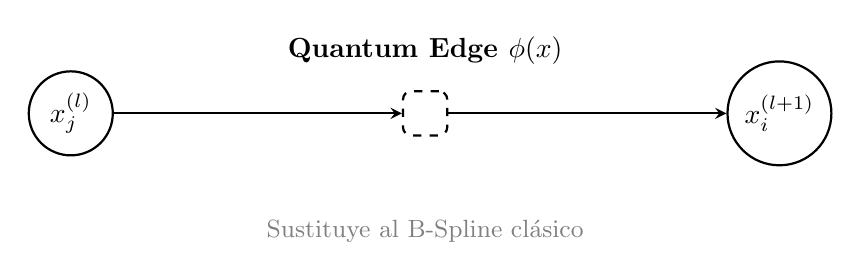
\begin{tikzpicture}
        % --- Nodos de la red neuronal (Izquierda y Derecha) ---
        \node[draw, circle, minimum size=0.8cm, thick] (Input) at (0,0) {$x_j^{(l)}$};
        \node[draw, circle, minimum size=0.8cm, thick] (Output) at (9,0) {$x_i^{(l+1)}$};
        
        % --- El circuito cuántico en el medio (Usando la caja guardada) ---
        % Nombramos a este nodo "Caja" para referenciarlo después
        \node[draw, dashed, thick, inner sep=8pt, rounded corners=3pt, 
              label={[yshift=0.2cm]above:\textbf{Quantum Edge $\phi(x)$}}] 
              (Caja) at (4.5,0) {\usebox{\circuitbox}};
        % --- Flechas de conexión ---
        % Conectamos dinámicamente desde el Input al borde Oeste de la Caja
        \draw[->, thick, >=stealth] (Input) -- (Caja.west);
        % Conectamos dinámicamente desde el borde Este de la Caja al Output
        \draw[->, thick, >=stealth] (Caja.east) -- (Output);
        % --- Anotación inferior ---
        \node[text=gray, font=\small] at (4.5, -1.5) {Sustituye al B-Spline clásico};
        
    \end{tikzpicture}
    
    \caption{Arquitectura de una arista en la Q-KAN. La función de activación 
    univariada $\phi(x)$ se implementa mediante un circuito cuántico variacional 
    (PQC) que codifica la entrada en una rotación $R_x$ y aprende los parámetros 
    en $R_y$.}
    \label{fig:quantum_kan_sketch}
\end{figure}

En esta arquitectura (ver Fig. \ref{fig:quantum_kan_sketch}), la transformación 
$\phi(x)$ en cada arista de la red se realiza mediante un pequeño circuito cuántico:

\begin{equation}
    \phi_Q(x; \boldsymbol{\theta}) = \langle 0 | U^\dagger(x, \boldsymbol{\theta}) 
    M U(x, \boldsymbol{\theta}) | 0 \rangle
\end{equation}

Donde:
\begin{itemize}
    \item $U(x, \boldsymbol{\theta})$ es un circuito que codifica el dato de 
    entrada $x$ (mediante rotaciones $R_x(x)$) y aplica capas variacionales 
    parametrizadas por $\boldsymbol{\theta}$.
    \item $M$ es un observable, por ejemplo $\sigma_z$.
    \item La salida del circuito es el valor escalar transformado.
\end{itemize}

\textbf{Implementación Esquemática en PennyLane:}
\begin{lstlisting}[language=Python, caption=Pseudocódigo para una capa Q-KAN usando PQC.]
@qml.qnode(dev, interface='tf')
def quantum_activation(inputs, weights):
    # Codificación de datos
    for i in range(n_qubits):
        qml.RX(np.pi * inputs[i], wires=i)
    
    # Capa Variacional (sustituye al Spline)
    for i in range(n_qubits):
        qml.RY(weights[i], wires=i)
    
    # Entrelazamiento (Captura correlaciones)
    for i in range(n_qubits-1):
        qml.CNOT(wires=[i, i+1])
        
    return [qml.expval(qml.PauliZ(i)) for i in range(n_qubits)]
\end{lstlisting}

\subsubsection{Ventajas Esperadas}
\begin{itemize}
    \item \textbf{Expresividad en el espacio de Hilbert:} 
    Un PQC puede generar funciones de activación con series de Fourier mucho más 
    ricas que un simple spline polinómico, capturando frecuencias más altas de 
    los datos con menos parámetros.
    \item \textbf{Paralelismo Cuántico:} La evaluación de las funciones $\phi$ en 
    superposición podría ofrecer ventajas de velocidad en hardware cuántico real.
\end{itemize}

\section{Conclusiones finales}

El desarrollo de las tareas de evaluación para GSoC 2025 ha permitido una 
exploración profunda en la intersección de la inteligencia artificial y la 
computación cuántica.
\begin{enumerate}
    \item Se demostró la competencia técnica en la manipulación de estados 
    cuánticos mediante \textbf{Cirq y PennyLane}, herramientas esenciales para 
    el diseño de algoritmos.
    \item La implementación de \textbf{Graph Neural Networks, GNNs,} para la 
    clasificación de jets confirmó que respetar la geometría intrínseca de los 
    datos físicos mejora significativamente la precisión frente a métodos 
    agnósticos a la estructura.
    \item Finalmente, la exploración de las \textbf{Redes Kolmogorov-Arnold (KANs)} 
    reveló un camino prometedor hacia modelos más interpretables. La propuesta 
    original de esta tesis, la \textbf{Q-KAN}, busca unificar estos mundos: 
    utilizar la estructura topológica de las KANs para mitigar la complejidad de 
    los circuitos cuánticos profundos, ofreciendo una arquitectura híbrida robusta 
    para la física de altas energías en la era NISQ.
\end{enumerate}